\chapter{Anwendung von Machine Learning in Videospielen}\label{ml_games_beispiele}
Obwohl klassische Machine Learning-Verfahren bereits seit Jahrzenten und damit schon vor der Popularisierung von Videospielen existierten, gab es bis vor kurzem nur wenige Spiele, die tatsächlich Gebrauch von Machine Learning gemacht haben. Im folgenden Kapitel werden Beispiele für die Anwendung von Machine Learning in Videospielen aufgezeigt um das Potential, das in dem Bereich besteht, hervorzuheben. Die genannten Anwendungsfälle beschränken sich nicht nur auf die Entwicklung intelligenter Agenten, sondern umfassen verschiedene Lösungen für die Erzeugung einer authentischeren Spielwelt.

% generelles:  https://hub.packtpub.com/uses-of-machine-learning-in-gaming/
% generelles: https://www.logikk.com/articles/machine-learning-in-game-development
% genrelles und story: https://developer.ibm.com/articles/machine-learning-and-gaming/
% generelles: integrating ML into a game
    % https://hackernoon.com/integrating-machine-learning-into-game-development-c5a7f31ed839

\section{Lernende Agenten}
Hier kann zwischen zwei Arten unterschieden werden, um das zugrundeliegende Modell, das die Entscheidungen der Agenten bestimmt, zu trainieren.
Zum einen gibt es Agenten, deren Modelle zur Laufzeit trainiert werden, also während des Spielens. Zum anderen kann schon zur Entwicklungszeit des Produkts ein Modell trainiert werden, das anschließend nicht mehr verändert wird.



\subsection{Lernen zur Laufzeit}
Lernende Agenten können zur Laufzeit trainiert werden, um die \ac{ki} so anzupassen, dass sie sinnvoll auf die Spielweise des Spielers reagieren kann.
Man könnte sich ein typisches \Fachbegriff{Stealth Game} vorstellen, in dem der Spieler über verschiedene mögliche Wege in ein Haus eindringen kann und sich dabei möglichst unauffällig verhalten muss. Das Haus wird von Wachen beschützt, die in bestimmten Intervallen um das Haus patroullieren. Diese Agenten der Wachen könnten nun das durch das Verhalten des Spielers trainiert werden, sodass sie beispielsweise häufige Laufwege oder weitere Spieltaktiken kontern können.
In derartigen Spielen verhalten sich NPCs normalerweise statisch, sodass ein Level sozusagen \sogenannt{auswendig gerlernt} werden kann. Sobald eine gute Lösung für ein Level gefunden wurde, kann dieser Vorgang wiederholt werden, um das Level immer auf die gleiche Art und Weise zu lösen. Einige Spiele versuchen dann, das statische Verhalten von NPCs zu überdecken, indem Zufallsvariablen verwendet werden. Wenn die Wachen allerdings zur Laufzeit lernen, den Spieler zu kontern, entsteht ein deutlich dynamischeres System und eine höhere Wiederspielbarkeit, da der selbe Ansatz nicht immer zum selben Ergebnis führt. Der Spieler muss dann kreativ werden und sich neue Lösungsansätze überlegen.



\subsubsection{Echo}
Im Spiel \Fachbegriff{Echo} \cite{echo} hingegen werden tatsächlich lernende Agenten benutzt, um ein ähnliches Szenario zu realisieren. Der Spieler tritt gegen eine Menge von Entitäten an, die das Verhalten des Spielers imitieren. Es werden sozusagen \Fachbegriff{Klone} des Spielers erzeugt. Wenn alle Klone besiegt wurden verdunkelt sich nach einer gewissen Zeit die Spielwelt. Dem Spieler ist bewusst, dass dies ein Hinweis darauf ist, dass während des Zeitraums der Verdunklung "verbesserte Versionen" der Klone hergestellt werden. Tatsächlich wird ein Machine Learning-Verfahren genutzt, um in dieser Zeit Agenten zu trainieren, die das Verhalten des Spielers erlernt haben \cite{echo_interview}. Je nachdem wie starr die Spielweise des Spielers ist, muss dieser anschließend in gewissem Maße \sogenannt{gegen sich selbst} kämpfen. Ein möglichst diverser Spielstil wird damit also gefördert.

\subsubsection{Black \& White}
% hier könnte noch mehr info sein!
% https://www.cs.rochester.edu/~brown/242/assts/termprojs/games.pdf
Bereits im Jahr 2001 wurde im Spiel \Fachbegriff{Black \& White} \cite{black-and-white} eine Kombination aus \Fachbegriff{Reinforcement Learning} (siehe Abschnitt \ref{reinforcement_learning})  und \Fachbegriff{Imitation Learning} (siehe Kapitel \ref{imitation_learning}) verwendet. Dabei handelt es sich um ein Strategiespiel, in dem der Spieler die Rolle eines Gottes einnimmt, der über ein Volk herrscht. Dieser kann sich entscheiden, ein guter oder ein böser Herrscher zu sein. Weiterhin befehligt der Spieler eine Kreatur, die seinen Stellvertreter in der Welt darstellt.
Mithilfe eines neuronalen Netzes imitiert diese Kreatur die Aktionen des Gottes und tendiert je nach Spielweise dazu, gut oder böse zu agieren. Weiterhin hat der Spieler die Möglichkeit, das Training direkt zu beeinflussen, indem er sie für bestimmte Aktionen bestraft oder belohnt, was sich auf die Moral der Kreatur auswirkt. Konkret wurde der Output des neuronalen Netzes, das für das Reinforcement Learning verwendet wurde, für die Anpassung eines Decision Trees verwendet, der die weitere Entscheidungsstrategie der Kreatur beeinflusst \cite{black-and-white_2}.

\subsubsection{Vorteile}
Die genannten Beispiele zeigen, dass durch das Anlernen von Agenten zur Laufzeit die Möglichkeit geschaffen wird, sehr interessante und dynamische Spielerlebnisse zu erschaffen. Agenten können auf Aktionen des Spielers mit einer Änderung ihres eigenen Verhaltens reagieren, was mit einem vortrainierten Modell nicht möglich ist. Das Trainieren des Modells kostet allerdings zusätzliche Leistung während der Ausführung des Spiels. 



\subsection{Nutzung vortrainierter Modelle}
Eine weitere Möglichkeit ist das Trainieren von lernenden Agenten vor der Laufzeit, zum Beispiel schon während der Entwicklungsphase eines Produkts. Das kann dann sinnvoll sein, wenn man dem Agenten objektive \sogenannt{richtige} und allgemeingültige Entscheidungen in Abhängigkeit seiner Inputparameter beibringen möchte. Das Verhalten des Agenten verändert sich zur Laufzeit nicht mehr. Daher eignet sich dies beispielsweise für die Realisierung von NPC-Gegnern in Strategiespielen, in denen durch das verwendete, erweiterte \sogenannt{Schere-Stein-Papier}-Prinzip Entscheidungen oft offensichtlich sind und nicht an das Verhalten des Spielers angepasst werden müssen.


\subsubsection{Forza Motorsport}
Ein weiteres Anwendungsbeispiel für Agenten, die vom Spieler selbst lernen, ist die bereits erwähnte Rennspielreihe \Fachbegriff{Forza Motorsport} \cite{forza}. Hier wird das Verhalten des Spielers genutzt, um einen Agenten mit Imitation Learning zu trainieren, mit dem sich der Spieler selbst messen kann \cite{forza_article}. Er fährt also Rennen gegen sich selbst, um sich zu verbessern und seine Fehler zu erkennen. Es ist auch möglich, Rennen gegen die \sogenannt{virtuellen Versionen} anderer Personen, genannt \sogenannt{Drivatar} von Freunden zu fahren, da die Drivatars in einer Cloud gespeichert werden \cite{forza_dev_video}.


\subsubsection{Supreme Commander 2}
Im Spiel \Fachbegriff{Supreme Commander 2} \cite{supreme_commander} werden gegnerische NPC-Agenten durch ein neuronales Netz gesteuert \cite{supreme_commander_gdc}. Genauer befasst sich die \ac{ai} mit der Auswahl sinnvoller Aktionen für das Kampfsystem. Es sollte daher betont werden, dass nicht das gesamte NPC-System auf Machine Learning basiert, sondern nur ein Teilaspekt davon, der allerdings für dieses spezifische Spiel essentiell ist.
Für die Kampfsysteme der verschiedenen Typen von Einheiten wurde dafür jeweils ein eigenes neuronales Netz trainiert. Es handelt sich um Land-, Luft-, Marine-, und Bombereinheiten. Jedes der neuronalen Netze verfügt über 34 Eingangsneuronen, die mit Inputdaten wie der Geschwindigkeit oder der Lebenspunkte der Einheit gespeist werden. Wenn sich zwei Gruppen gegenerischer Einheiten gegenüberstehen, werden hierfür Differenzen aus den jeweiligen Werten gebildet. Dieser Vorgang wurde in einer Präsentation des Lead Developers Mike Robbins auf der \ac{gdc} \cite{gdc} im Jahre 2012 näher erläutert.
Es wird eine einzelne \Fachbegriff{Hidden Layer} verwendet, die 98 Neuronen beinhaltet. Die Outputschicht verfügt über 15 Neuronen, die jeweils eine mögliche Aktion für die Einheit darstellen. Dabei handelt es sich um taktische Entscheidungen, wie beispielsweise \sogenannt{Attack Closest} oder \sogenannt{Attack Weakest}. Damit die Agenten dazulernen, wird beim Training die sogenannte \sogenannt{Fitness} der involvierten Einheiten betrachtet. Diese Metrik wird analysiert, indem alle Inputvariablen des Netzes nach der durchgeführten Aktion erneut betrachtet und Differenzen zu den vorherigen Werten gebildet werden. So kann entschieden werden, welcher Agent einen Kampf gewonnen hat. Durch \Fachbegriff{Backpropagation} oder auch \Fachbegriff{Fehlerrückführung} werden anschließend Gewichtungen innerhalb des neuronalen Netzes vorgenommen. Laut Robbins werden die Netze anschließend für jeweils eine Stunde trainiert.

Auch im komplexeren inoffiziellen Nachfolgerspiel von Supreme Commander 2, \Fachbegriff{Plantary Annihilation} \cite{pa_game}, wurde ein solches Verfahren verwendet \cite{pa_game_forum}. Die Dimensionen dieses Spiels übersteigen die des Vorgängers erheblich. Der Spieler kann auf einer Mehrzahl unabhängiger Planeten gleichzeitig agieren und tausende Einheiten gleichzeitig kommandieren. Damit wird gezeigt, dass Machine Learning-Verfahren eine hohe Skalierbarkeit aufweisen können.

\subsubsection{Vorteile}
Im Vergleich zur Nutzung von Agenten, die erst während des tatsächlichen Spielvorgangs trainiert werden, liegt laut Robbins ein Performancevorteil vor. Durch das Wegfallen dieses Trainingsvorgangs zur Laufzeit können mehr Ressourcen für die Darstellung des Spiels verwendet werden. Abhängig vom Spiel seien auch ausreichend vortrainierte Modelle in der Lage, allgemeingültige und objektiv richtige Entscheidungen unabhängig vom Spieler zu fällen, sodass ein Trainingsvorgang während der Laufzeit nicht zwangsweise ein besseres Ergebnis erziele.



\section{Anwendungsfälle außerhalb der intelligenten Agenten}
% https://towardsdatascience.com/neural-networks-and-the-future-of-3d-procedural-content-generation-a2132487d44a
% https://aifrontiers.com/2018/09/20/an-overview-of-artificial-intelligence-for-video-games/
Dieser Abschnitt befasst sich zusätzlich mit weiteren Anwendungsfällen, die außerhalb des Bereichs der Entwicklung von intelligenten Agenten liegen. Im Allgemeinen wird maschinelles Lernen eingesetzt, um überlegende Technologien und Inhalte zu entwickeln. Häufig dient es aber auch als ein Mittel für das Einsparen von Kosten durch die prozedurale Generierung von Inhalten. Die Nutzung solcher Methoden bietet nicht nur das Potential, verbesserte Spielerlebnisse zu erzeugen, sondern ebenfalls die Möglichkeit einer erheblichen Kostensenkung durch die nicht länger bestehende Notwendigkeit zur Beschäftigung großer Mengen von beispielsweise Level- oder Game Designern.

\paragraph{Prozedurale Generierung}
Ein klassischer Anwendungsfall für prozedurale Generierung ist die Erzeugung von \Fachbegriff{Height Maps} und Terrain, etwa durch Rauschfunktionen wie \Fachbegriff{Perlin Noise} \cite{minecraft_perlin} \cite{ml_procedural_article}. Ein bekanntes Beispiel ist das erfolgreiche Spiel Minecraft \cite{minecraft}. Kürzlich konnte gezeigt werden, dass ebenfalls mithilfe von \acp{gan} eine parametrisierbare prozedurale Generierung ganzer Level umgesetzt werden kann \cite{mario_pcg}. Es werden bereits vorhandene Level genutzt, um neue Level zu erzeugen und anschließend aus der resultierenden latenten Menge ideale Level auszusuchen, die bestimmte Kriterien erfüllen.

\paragraph{Game Design}
Verschiedene Arbeiten demonstrieren darüber hinaus, dass auch der Teilbereich des Game Design, wie das \textit{Balancing} von Machine Learning übernommen werden kann \cite{balancing_reinforcement_1} \cite{balancing_reinforcement_2} \cite{balancing_reinforcement_3}. Mithilfe von Reinforcement Learning werden dabei bestimmte Parameter für gegnerische Agenten oder ganz direkt der Schwierigkeitsgrad des Spiels bestimmt. 

\paragraph{Bewegungen und Animationen}
Ein weiterer Bereich für potentielle Kostenreduzierungen ist die Erzeugung von \Fachbegriff{Character Content}. 2017 wurde von \texttt{Holden et al.} gezeigt, dass mithilfe von \Fachbegriff{Phase-Functioned Neural Networks} äußerst glaubwürdige Echtzeit-Charakteranimationen erzeugt werden können \cite{holden_paper} \cite{holden_github}. Frei verfügbare Motion Capturing-Datenbanken wie \Fachbegriff{MoCap} von der Carnegie Mellon University \cite{mocap} können als Trainingsdaten dienen und erleichtern derartige Verfahren zusätzlich. NVidia und Remedy Entertainment haben ebenfalls 2017 erfolgreich gezeigt, dass mit Trainingsdaten, die lediglich aus zwei zehnminütigen Videosequenzen bestehen, in Echtzeit realistisch wirkende Gesichtsanimationen erzeugt werden können, die ausschließlich auf Audiodaten basieren \cite{nvidia_face_paper} \cite{nvidia_face_website}. Dabei wurde das Ziel verfolgt, den Sprechstil einer einzelnen Person zu modellieren. Dieses wurde deutlich überschritten, da mit den verwendeten \Fachbegriff{Deep Learning}-Methoden selbst Geschlechter, Sprachen und Akzente abgebildet werden können.
Square Enix hat weiterhin bereits 2013 gezeigt, dass Reinforcement Learning verwendet werden kann, um einen Charaktercontroller zu entwerfen \cite{hitman_gdc}. Dieser wurde im Rahmen des Spiels \Fachbegriff{Hitman: Absolution} \cite{hitman} entwickelt und verwendet. Damit wird gezeigt, dass Machine Learning auch in anderen Bereichen zur Verbesserung intelligenter Agenten beitragen kann. Neben den Entscheidungen, die ein solcher Agent trifft, ist auch die audiovisuelle Wirkung von hoher Bedeutung für die Authentizität und den erreichten Grad von Realismus und Immersion.


\paragraph{Testing und Analytics}
Machine Learning kann weiterhin für Test- oder Analysezwecke verwendet. In der Regel werden dann im Hintergrund oder im Backend Dienste genutzt, die dem Spieler nicht bekannt sind. Häufig stellen sich hier Klassifizierungsaufgaben, bei denen Aussagen über das Spielerverhalten getroffen werden sollen. Für eine beispielhafte Firma, die Onlinespiele vermarktet, kann es etwa vorteilhaft sein, Aussagen über das zukünftige Spielerverhalten treffen zu können - beispielsweise wann ein Spieler mit dem Spielen aufhört. Dieser kann dann explizit durch Marketingmaßnahmen anvisiert werden.
Ein weiteres Anwendungsfeld ist das Durchführen von Usertests, die typischerweise in der Entwicklungsphase von Spielen durchgeführt werden, um potentielle Defizite in verschiedenen Bereichen zu identifizieren. So können etwa anhand der Dauer, die Spieler an  bestimmten Orten verbringen, Heatmaps erstellt werden, um Probleme im Level- oder Game Design aufzudecken. Derartige Tests können durch Machine Learning-gestützte Verfahren verbessert werden, indem beispielsweise die Gesichtsausdrücke eines Spielers identifiziert werden, um Informationen zu seiner Stimmung zu erhalten.
Derartige Vorhersagen sind auch für die Verwendung im eigentlichen Spiel selbst denkbar. Das Spielverhalten könnte analysiert werden, um beispielsweise den Schwierigkeitsgrad automatisch anzupassen oder Vorlieben des Spielers in die Generierung von prozeduralen Inhalten mit einzubeziehen.




\section{Aktuelle Entwicklungen}\label{aktuelle_entwicklungen_rl}
In diesem Abschnitt werden aktuelle Entwicklungen im Bereich von \ac{reinforcement_learning} ausgeführt. Heutzutage ist vermehrt zu beobachten, dass das Verfahren für die Realisierung kompetitiver Agenten in bereits fertigen Spielen verwendet wird, die gegen echte Spieler antreten. Neueste Projekte wie \Fachbegriff{AlphaZero} \cite{google_deep_mind} und \Fachbegriff{OpenAI Five} \cite{openai_five_paper} beweisen, dass \ac{reinforcement_learning} über ein großes Potential verfügt. Die folgenden Beispiele zeigen, dass komplexe Verhaltensmuster entstehen und übermenschliche Leistungen erreicht werden können.
% Dies wird schon in 3_3 behandelt oder nicht?!?
% OpenAI 5 etc.
    % INTELLIGENTE AGENTEN LERNEN, FERTIGE SPIELE ZU SPIELEN (api oder controller emulator?)
    % https://emerj.com/ai-sector-overviews/machine-learning-in-gaming-building-ais-to-conquer-virtual-worlds/
    % minecraft http://minerl.io/


\subsection{DeepMind}
Der Firma DeepMind Technologies, einer Tochter von \Fachbegriff{Alphabet Inc.}, ist es mit seiner KI \Fachbegriff{AlphaZero} \cite{deepmind_alphazero} \cite{google_deep_mind} gelungen, traditionelle Brettspiele wie Schach, Jogi und Go zu meistern und selbst Weltmeister darin zu schlagen. Der seit 2013 amtierende Schachweltmeister Magnus Carlsen selbst behauptet, AlphaZero sei zu gut, um emuliert zu werden oder ihren Stil nachzuahmen \cite{carlsen_chess}.

Weiterhin hat DeepMind einen Agenten entwickelt, der mit Deep Reinforcement Learning einen Großteil aller Spiele der Atari-Konsole meistert \cite{deepmind_atari_paper}. Dafür wurde ein Convolutional Neural Network verwendet, das mit einer Variante von Q-Learning arbeitet (siehe Abschnitt \ref{q-learning}). Der Input des Netzes besteht lediglich aus den auf dem Bildschirm zu sehenden Pixeln. Der Output stellt die Steuerung des Charakters dar, so wie sie auch über einen Controller möglich wäre. Die Besonderheit ist dabei, dass der Agent ohne eine Anpassung der Architektur oder des Lernalgorithmus in der Lage ist, eine Vielzahl von Spielen zu beherrschen. Konkret wurde das Verfahren mit sieben Spielen getestet, wobei in drei Fällen eine übermenschliche Performance des Agenten erreicht wurde, obwohl lediglich Pixel als Beobachtungen verwendet wurden.

\subsection{OpenAI Five}
Die Firma OpenAI LP arbeitet an vergleichbaren Projekten, allerdings auch im Bereich von Online-Games und E-Sports. Das Spiel \Fachbegriff{Dota 2} \cite{dota_2} wird von OpenAI seit 2016 als Plattform für KI-Forschung verwendet. In dem komplexen Spiel treten zwei Teams aus jeweils fünf Helden mit einer Vielzahl von Fähigkeiten und möglichen Aktionen gegeinander an. In diesem Rahmen wurde eine ebenfalls auf \ac{reinforcement_learning} basierende KI mit dem Namen \Fachbegriff{OpenAI Five} entwickelt \cite{openai_five} \cite{openai_five_paper}. OpenAI Five übernimmt dabei die Kontrolle über alle fünf Charaktere eines Teams. Im Jahr 2018 schaffte es die KI nur fast, zwei professionelle E-Sports Teams zu schlagen. Im Dezember 2019 hingegen gelang ihr ein eindeutiger Sieg über das aktuelle Weltmeisterteam. Dieser Fortschritt zeigt, dass die KI selbst nach jahrelangem Training noch deutlich verbessert werden konnte.
Das Training der Agenten findet in einer beschleunigten virtuellen Dota2-Umgebung statt. Dabei spielt die KI stets gegen sich selbst und hat umgerechnet bereits mehr als 10.000 Jahre Spieleerfahrung gesammelt. Die Observations der Agenten entsprechen den Informationen, die auch ein menschlicher Spieler auf seinem Bildschirm sehen würde. Ebenso verhält es sich mit den möglichen auswählbaren Aktionen.

Folgende Umstände waren bei der Entwicklung der KI problematisch:
\begin{itemize}
    \item \texttt{Langfristiger Zeithorizont}: Bei einer angenommenen Serverframerate von 30 Hz und einer Länge von durchschnittlich 45 Minuten mit Entscheidungen, die jeden vierten Frame getroffen werden ergeben sich insgesamt etwa 20.000 Aktionen pro Spiel. Zum Vergleich liegt diese Zahl beim Schach bei etwa 80 und in dem Brettspiel \Fachbegriff{GO} bei etwa 150.
    \item \texttt{Eingeschränkt sichtbarer Spielzustand}: Spieler und Agent können nur in einem begrenzten Bereich um den Charakter Objekte wie Feinde, etc. wahrnehmen.
    \item \texttt{Hochdimensionaler kontinuierlicher Observations- und Handlungsraum}: Mit dutzenden Spielern, NPCs, Gebäuden und Fähigkeiten stehen dem Agenten zu jedem Zeitpunkt etwa 1.000 von rund 170.000 möglicher verschiedener Aktionen zur Verfügung. Zusätzlich werden etwa 20.000 Werte aus der Umgebung als relevante Beobachtungen für Entscheidungen verwendet.
\end{itemize}


Diese Hürden wurden durch ein Deep Learning-Verfahren gemeistert, dessen zugrunde liegendes rekurrentes neuronales Netz über 159 Millionen Neuronen verfügt. Dabei wurde der \ac{ppo}-Algorithmus verwendet (siehe Kapitel \ref{proximal_policy_optimization}), der auch in dieser Thesis verwendet wird. Zusätzlich wird ein \Fachbegriff{Long short-term memory} \cite{lstm} mit einer Schicht und 4096 Einheiten verwendet, mit dem den Agenten ein Gedächtnis verliehen wird.
Die Policy, die zum Sieg über den Dota 2-Welmeister geführt hatte, ergab sich nach einem zehn Monate andauernden Trainingsvorgang unter Nutzung von Proximal Policy Optimization bei einer durchschnittlichen neuronalen Rechenleistung von 770 PFlops/s-days, oder \Fachbegriff{pfs-day} \cite{openai_compute_blog}. Ein pfs-day entspricht einer Rechenleistung von $10^{15}$ neuronalen Rechenoperationen pro Sekunde für eine Dauer von einem Tag. Verglichen mit AlphaGO wurden 20 mal so viele Neuronen verwendet und 25 mal so viel Trainingszeit aufgebracht. Dadurch hat sich der in Abbildung \ref{fig:trainingsverlauf_openai} zu sehende Trainingsverlauf ergeben.


\begin{figure}[H]
\centering
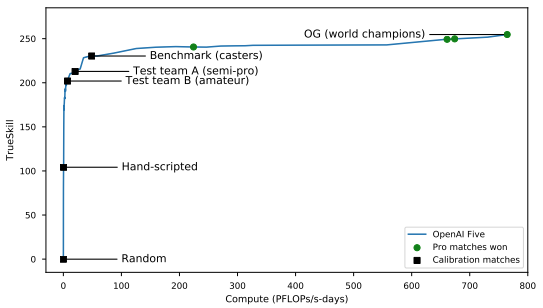
\includegraphics[scale=0.65]{images/trainingsverlauf_openai.png}
\caption{Trainingsverlauf OpenAI Five \cite{openai_five_paper}}
\label{fig:trainingsverlauf_openai}
\end{figure}

Bei dem auf der y-Achse verzeichneten \Fachbegriff{TrueSkill}-Wert handelt es sich um eine im Jahr 2007 vorgestellte Metrik für die Einschätzung des Skill-Levels in kompetitiven Spielen \cite{NIPS2006_3079}. Die Grafik zeigt einen zunächst drastischen Anstieg aufgrund der exponentiellen Natur des Problems, sodass bereits nach sehr kurzer Zeit semiprofessionelle Teams geschlagen werden konnten. Das ist bereits eine sehr aussagekräftige Metrik, da auch semiprofessionelle menschliche Spieler jahrelanges intensives Training absolvieren müssen, um dieses Level zu erreichen. Der anschließende Verlauf ist nur sehr leicht steigend. Verbesserungen zum Ende des Verlaufs wurden mit der Einführung weiterer Fähigkeiten, die der KI zuvor nicht verwenden konnte, begründet, sodass schließlich auch das aktuell beste menschliche Team geschlagen werden konnte.

Es zeigt sich, dass selbst überaus komplexe Spiele und damit schwierige Probleme mit \ac{reinforcement_learning} gemeistert werden können. Sie beweisen zum Einen die Skalierbarkeit klassischer Machine Learning-Methoden und zum Anderen die Möglichkeit, Agenten in Verbindung mit einer großen Menge von Rechenleistung übermenschliche Fähigkeiten zu verleihen. Dabei dienen Videospiele als eine Art \sogenannt{Spielplatz} für das Experimentieren und Forschen mit Machine Learning-Verfahren, da diese eine optimale Umgebung dafür bieten.


%- openAI hide and seek --> sehr interessante, unerwartet verhaltensmuster

% Hide and seek
    % https://www.quantamagazine.org/artificial-intelligence-discovers-tool-use-in-hide-and-seek-games-20191118/


% neuer ansatz: statt experience learning multi agent ansatz:
% http://proceedings.mlr.press/v48/mniha16.pdf

% https://hciweb.iwr.uni-heidelberg.de/system/files/private/downloads/541645681/dammann_reinfocement-learning-report.pdf


%- veränderung in den letzten jahren?
%- altbewährte systeme wie decision trees immernoch nützlich?


\section{Potential}
Die oben genannten Beispiele zeigen, dass es eine Vielzahl von Anwendungsfällen für Machine Learning in Videospielen gibt. Neben der Verbesserung intelligenter Agenten sind auch andere Bereiche relevant, die zur Erschaffung von Welten mit einer erhöhten Glaubwürdigkeit und Authentizität beitragen können. Die genannten Spiele zeigen, wie kreativ lernende Agenten in sehr unterschiedlichen Bereichen eingesetzt werden können und welche interessante Szenarien damit vorstellbar sind. Die Nutzung in Strategiespielen beweist darüber hinaus die Skalierbarkeit der Verfahren. Sie ermöglichen eine Interaktion mit dem Spieler, die mit klassischen Verfahren nicht realisierbar ist und erzeugen so authentische Spielerlebnisse.

Der Entwickler von \Fachbegriff{Supreme Commander 2} und \Fachbegriff{Planetary Annihilation}, nennt eine Menge von Vorteilen, die sich direkt aus der Nutzung eines neuronalen Netzes ergeben:

\begin{itemize}
    \item \texttt{Gewichtung der Inputs}: Eine Gewichtung der Inputs fällt weg.
    \item \texttt{Wichtigkeit der Inputs irrelevant}: Wenn irrelevante Inputs vorhanden sind, sollte das System davon nicht beeinflusst werden.
    \item \texttt{Vergleichbarkeit der Zustandsvariablen}: Es ist nicht nötig, die einzelnen Werte miteinander zu vergleichen. Wäre dies nicht der Fall, so müsste ein Weg gefunden werden, um beispielsweise Inputvariablen wie \textit{Geschwindigkeit} und \textit{Schaden} vergleichen zu können.
    \item \texttt{Kein Algorithmus nötig}: Es muss kein Algorithmus entwickelt werden, der das genaue Verhalten der Einheiten beschreibt.
\end{itemize}

Laut Robbins bestehe ein großer Vorteil also darin, dass fast beliebige Werte als Inputvariablen für das neuronale Netz verwendet werden können. Das neuronale Netz kümmere sich dann anstelle des Entwicklers von selbst um die Normalisierung und den Vergleich der Variabeln. Weiterhin sei es nicht nötig das Verhalten der Agenten direkt zu beschreiben, sodass insgesamt viel Arbeitszeit gespart wird.

Im Allgemeinen können außerdem Kosten gespart werden, indem Inhalte generiert werden, anstatt dafür einen hohen Arbeitsaufwand aufzubringen. Besonders bei der Nutzung intelligenter Agenten besteht das Potential, den massiven Zeitaufwand des Scriptings zu reduzieren, indem beispielsweise Reinforcement Learning genutzt wird. Das Verhalten der Agenten muss dann nicht explizit definiert werden, weil es \Fachbegriff{erlernt} wird.
Die Menge der Inhalte, die für ein erfolgreiches Spiel nötig sind, sollten dabei nicht unterschätzt werden. Im 2018 erschienenen Spiel \Fachbegriff{Red Dead Redemption 2} \cite{rdr2} wurden allein etwa 300.000 Charakter- und Tieranimationen angefertigt bzw. aufgenommen \cite{rdr2_script_pages}. Dadurch kann ein guter Eindruck darüber gewonnen werden, wie viel Zeit und Geld durch eine prozedurale Generierung von Animationen gespart werden könnte.
Aktuelle Entwicklungen beweisen ein vielversprechendes Potential, da selbst in komplexen Szenarien menschenähnliches oder sogar übermenschliches Verhalten erlernt werden kann. Reinforcement Learning zeigt, dass auch mit altbewährten Algorithmen erstaunliche Ergebnisse erreicht werden können, die in hohem Maße und durch den erhöhten Einsatz von leistungsfähiger Hardware skalierbar sind. Das lässt für die Entwicklung von NPCs vermuten, dass ebenfalls menschenähnliches Verhalten nachgeahmt werden kann, um die Immersion virtueller Welten zu erhöhen.